\documentclass[aspectratio=169, 10pt]{beamer}

% --- Language & Fonts ---
\usepackage[utf8]{inputenc}
\usepackage[T1]{fontenc}
\usepackage{lmodern}
\usepackage{FiraSans}
\usepackage{FiraMono}
\usepackage{microtype}

% --- Math & Science ---
\usepackage{amsmath, amssymb, amsfonts}
\usepackage{mathtools}
\usepackage{siunitx}
\usepackage{booktabs}
\usepackage{graphicx}
\usepackage{physics}

% --- Tikz ---
\usepackage{tikz}
\usepackage{pgfplots}
\pgfplotsset{compat=1.18}
\usetikzlibrary{calc}


\definecolor{conductionblue}{RGB}{220, 235, 252}
\definecolor{valencegreen}{RGB}{225, 245, 225}
\definecolor{electronred}{RGB}{215, 48, 39}
\definecolor{holeblue}{RGB}{44, 123, 182}

\definecolor{groundstate}{RGB}{44, 123, 182}
\definecolor{excitedstate}{RGB}{215, 48, 39}
\definecolor{photonred}{RGB}{230, 57, 70}
\definecolor{photonblue}{RGB}{29, 53, 87}

\definecolor{signalred}{RGB}{215, 48, 39}
\definecolor{gateblue}{RGB}{44, 123, 182}

\usetikzlibrary{shapes.geometric, arrows.meta, decorations.markings, calc}
% Required TikZ libraries:
\usetikzlibrary{decorations.pathmorphing, decorations, positioning, arrows.meta, circuits.ee.IEC}

% Define arrow decoration for beam paths
\tikzset{
  beam arrow/.style={
    postaction={
      decorate,
      decoration={
        markings,
        mark=at position 0.55 with {\arrow[red, thick]{Stealth[length=2.5mm]}}
      }
    }
  },
  beam arrow orange/.style={
    postaction={
      decorate,
      decoration={
        markings,
        mark=at position 0.55 with {\arrow[orange!90!black, thick]{Stealth[length=2.5mm]}}
      }
    }
  }
}


% --- Muted & Natural Color Palette ---
\definecolor{MutedCharcoal}{RGB}{44, 54, 63}   % #2C363F - Deep charcoal header
\definecolor{MutedSage}{RGB}{91, 112, 101}     % #5B7065 - Earthy sage accent
\definecolor{MutedClay}{RGB}{197, 123, 87}     % #C57B57 - Muted terracotta/amber
\definecolor{MutedText}{RGB}{58, 61, 64}       % #3A3D40 - Soft off-black text
\definecolor{PaperBg}{RGB}{247, 246, 242}      % #F7F6F2 - Warm off-white paper canvas
\definecolor{CardBg}{RGB}{255, 255, 255}       % Clean white card background
\definecolor{SubtleGray}{RGB}{140, 145, 150}   % Muted gray for footers

% --- Beamer Core Styling ---
\setbeamercolor{background canvas}{bg=PaperBg}
\setbeamercolor{normal text}{fg=MutedText}

% Title & Frame Headlines
\setbeamercolor{titlelike}{fg=MutedCharcoal}
\setbeamercolor{frametitle}{fg=MutedCharcoal, bg=PaperBg}
\setbeamerfont{frametitle}{size=\Large, series=\bfseries}

% Structure & Bullet points
\setbeamercolor{structure}{fg=MutedSage}
\setbeamertemplate{navigation symbols}{}
\setbeamertemplate{items}[circle]

% --- Muted Blocks Styling ---
\setbeamercolor{block title}{fg=white, bg=MutedCharcoal}
\setbeamercolor{block body}{fg=MutedText, bg=CardBg}

\setbeamercolor{block title example}{fg=white, bg=MutedSage}
\setbeamercolor{block body example}{fg=MutedText, bg=CardBg}

\setbeamercolor{block title alert}{fg=white, bg=MutedClay}
\setbeamercolor{block body alert}{fg=MutedText, bg=CardBg}

\setbeamertemplate{blocks}[rounded][shadow=false]

% --- Subtle Footer ---
\setbeamertemplate{headline}{} % Leave headline clean

% Frame Title Layout (Title Top-Left, Logo Top-Right)
\setbeamercolor{frametitle}{fg=MutedCharcoal, bg=PaperBg}
\setbeamerfont{frametitle}{size=\Large, series=\bfseries}

\setbeamertemplate{frametitle}{%
  \nointerlineskip%
  \begin{beamercolorbox}[wd=\paperwidth, ht=4.5ex, dp=1ex, leftskip=2ex, rightskip=2ex]{frametitle}%
    \usebeamerfont{frametitle}\insertframetitle%
    \hfill%
    \raisebox{-0.15cm}{
\includegraphics[height=1cm]{img/UU_logo_2021_EN_BLACK.png}}% Replace with logo.png
  \end{beamercolorbox}%
}

\setbeamertemplate{footline}{
  \leavevmode%
  \hbox{%
    \begin{beamercolorbox}[wd=.333333\paperwidth,ht=2.5ex,dp=1.125ex,left]{author in head/foot}%
      \usebeamerfont{author in head/foot}\hspace*{2ex}\textcolor{SubtleGray}{\insertshortauthor}
    \end{beamercolorbox}%
    \begin{beamercolorbox}[wd=.333333\paperwidth,ht=2.5ex,dp=1.125ex,center]{title in head/foot}%
      \usebeamerfont{title in head/foot}\textcolor{SubtleGray}{\insertshorttitle}
    \end{beamercolorbox}%
    \begin{beamercolorbox}[wd=.333333\paperwidth,ht=2.5ex,dp=1.125ex,right]{date in head/foot}%
      \usebeamerfont{date in head/foot}\textcolor{SubtleGray}{\insertframenumber{} / \inserttotalframenumber}\hspace*{2ex} 
    \end{beamercolorbox}%
  }%
  \vskip1ex
}

% --- Presentation Metadata ---
\title[Hot carrier-dynamics]{Hot carrier-dynamics}
\subtitle{Hot carrier-dynamics in Silicon single crystals}
\author[B.J. Spijkerman]{B.J. Spijkerman\inst{1}}
\institute[Utrecht University]{
  \inst{1}Utrecht University
}
\date{\today}

% --- Document Start ---
\begin{document}

% 1. Title Slide
{
\setbeamertemplate{footline}{}
\begin{frame}
  \titlepage
\end{frame}
}

% --- Section 1 ---
\section{Motivation \& Background}

\begin{frame}{Motivation \& Background}
  \begin{minipage}{0.48\textwidth}
    \begin{itemize}
      \item \textbf{Shockley-Quaser:} Thermodynamical limiting efficiency for solar panels.
      \item \textbf{Hot carrier-dynamics:} Very little known about hot state conductivity.
      \item \textbf{Photocurrent spectroscopy:} Measuring carrier-dynamics with pico-second resolution.
    \end{itemize}
  \end{minipage}\hfill
  \begin{minipage}{0.48\textwidth}
    \begin{figure}[!h]
      \centering
%      \includegraphics[width=\textwidth]{}
      \caption{}
    \end{figure}
  \end{minipage}
\end{frame}

% --- Section 2 ---
\section{Experimental Methods}

\begin{frame}{Photo- current/ conductivity Spectroscopy}
  \begin{minipage}{0.48\textwidth}
    \begin{itemize}
      \item Optical pump electrical probe
      \item Electrical detection
      \item Advantages over TA methods
    \end{itemize}
  \end{minipage}\hfill
  \begin{minipage}{0.48\textwidth}
    \begin{figure}[!h]
      \centering
      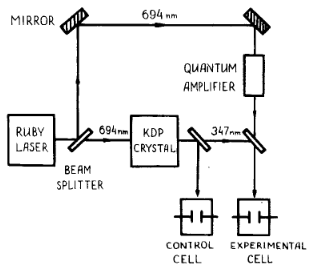
\includegraphics[width=\textwidth]{img/firstPCS.png}
    \end{figure}
    \vspace{-5mm}
    {\tiny\color{gray}{L.V Lukin, \textit{et all}, Chemical Physics Letters, Volume 81, Issue 3, 1981.}}
  \end{minipage}
\end{frame}


\begin{frame}{Experimental Methods}
  \begin{block}{Conductivity changes}
    The material responds to illumination by changing its conductivity:
    \begin{equation}
      \Delta\sigma=\Delta\mu\Delta N
    \end{equation}
  \end{block}

  \begin{columns}[T]
    \begin{column}{0.48\textwidth}
      \begin{exampleblock}{Key Properties}
        \begin{itemize}
          \item $\Delta\sigma=\Delta\sigma_1+\Delta\sigma_2+C(\tau)$
          \item $\mu$ is related to carrier-dynamics.
          \item $N$ is related to carrier-population.
        \end{itemize}
      \end{exampleblock}
    \end{column}

    \begin{column}{0.48\textwidth}
      \begin{alertblock}{Important Consideration}
        The different states have their own carrier mobility $\mu_i$.
        \begin{equation}
          \Delta\sigma=\sum_i\mu_iN_i - \sigma_0
        \end{equation}
      \end{alertblock}
    \end{column}
  \end{columns}
\end{frame}


\begin{frame}{Experimental Setup}
  \centering
  \resizebox{\textwidth}{!}{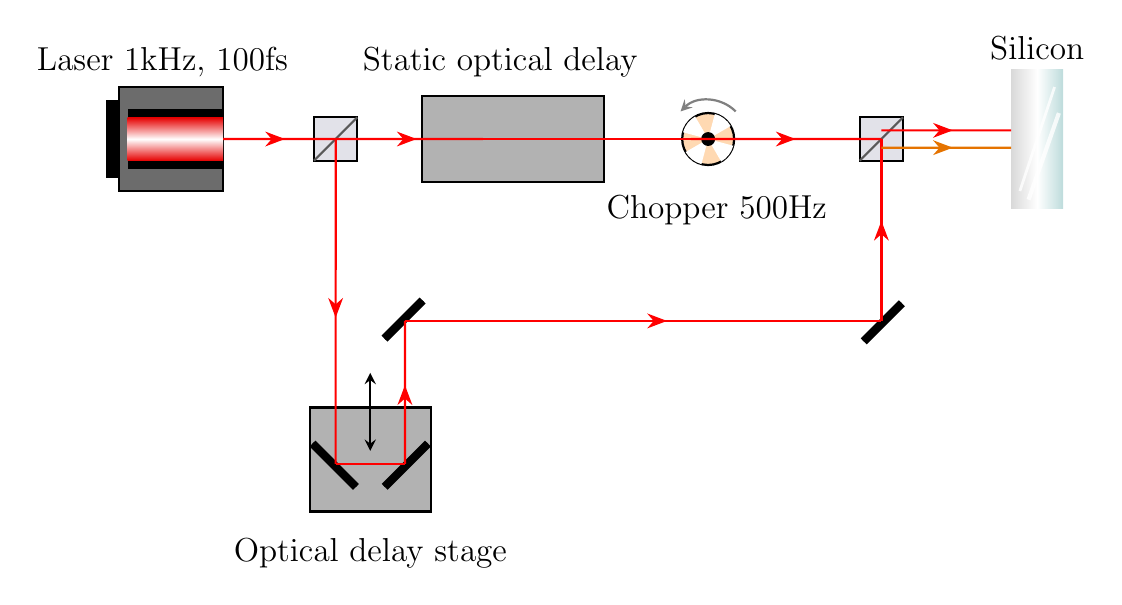
\begin{tikzpicture}[scale=1.1, >=stealth]

    % ==========================================
    % 1. LASER SOURCE
    % ==========================================
    % Label
    \node[anchor=south] at (0.5, 1.2) {\large Laser 1kHz, 100fs};
    
    % Main Body (Dark Box)
    \filldraw[fill=gray!85!black, draw=black, thick] (0, 0) rectangle (1.2, 1.2);
    % Rear Cap
    \fill[black] (-0.15, 0.15) rectangle (0, 1.05);
    % Inner Beam Chamber (Glow effect)
    \fill[black] (0.1, 0.25) rectangle (1.2, 0.95);
    \fill[top color=red!90!black, bottom color=red!90!black, middle color=white] (0.1, 0.35) rectangle (1.2, 0.85);

    % ==========================================
    % 2. BEAM SPLITTER 1 (Top Left)
    % ==========================================
    \coordinate (BS1) at (2.5, 0.6);
    \draw[thick, fill=blue!15!gray!20] ($(BS1)+(-0.25,-0.25)$) rectangle ($(BS1)+(0.25,0.25)$);
    \draw[thick, gray!70!black] ($(BS1)+(-0.25,-0.25)$) -- ($(BS1)+(0.25,0.25)$);

    % ==========================================
    % 3. STATIC OPTICAL DELAY (Top Middle)
    % ==========================================
    \node[anchor=south] at (4.4, 1.2) {\large Static optical delay};
    \filldraw[fill=gray!60, draw=black, thick] (3.5, 0.1) rectangle (5.6, 1.1);
    
    % ==========================================
    % 4. BEAM COMBINER / SPLITTER 2 (Top Right)
    % ==========================================
    \coordinate (BS2) at (8.8, 0.6);
    \draw[thick, fill=blue!15!gray!20] ($(BS2)+(-0.25,-0.25)$) rectangle ($(BS2)+(0.25,0.25)$);
    \draw[thick, gray!70!black] ($(BS2)+(-0.25,-0.25)$) -- ($(BS2)+(0.25,0.25)$);

    % ==========================================
    % 5. SILICON TARGET (Far Right)
    % ==========================================
    \node[anchor=south] at (10.6, 1.4) {\large Silicon};
    % Gradient Block
    \fill[left color=gray!30, right color=cyan!30!gray!40, middle color=white] (10.3, -0.2) rectangle (10.9, 1.4);
    % Glass Sheen Lines
    \draw[white, opacity=0.8, line width=1pt] (10.4, 0.0) -- (10.8, 1.2);
    \draw[white, opacity=0.8, line width=1.5pt] (10.5, -0.1) -- (10.85, 0.9);

    % ==========================================
    % 6. OPTICAL DELAY STAGE (Bottom Left)
    % ==========================================
    \node[anchor=north] at (2.9, -3.9) {\large Optical delay stage};
    \filldraw[fill=gray!60, draw=black, thick] (2.2, -3.7) rectangle (3.6, -2.5);
    
    % Retroreflector Mirrors inside Stage
    % Left mirror (45 deg)
    \coordinate (M_stage1) at (2.5, -3.15);
    \draw[ultra thick] ($(M_stage1)+(0.25,-0.25)$) -- ($(M_stage1)+(-0.25,0.25)$);
    \fill[black] ($(M_stage1)+(0.25,-0.25)$) -- ($(M_stage1)+(-0.25,0.25)$) -- ($(M_stage1)+(-0.3,0.2)$) -- ($(M_stage1)+(0.2,-0.3)$) -- cycle;
    
    % Right mirror (-45 deg)
    \coordinate (M_stage2) at (3.3, -3.15);
    \draw[ultra thick] ($(M_stage2)+(-0.25,-0.25)$) -- ($(M_stage2)+(0.25,0.25)$);
    \fill[black] ($(M_stage2)+(-0.25,-0.25)$) -- ($(M_stage2)+(0.25,0.25)$) -- ($(M_stage2)+(0.3,0.2)$) -- ($(M_stage2)+(-0.2,-0.3)$) -- cycle;

    % Delay Stage Double Arrow
    \draw[<->, thick] (2.9, -2.1) -- (2.9, -3.0);

% --- THE CHOPPER IN THE UPPER ARM ---
    % Placed midway between the Beam Splitter and the Upper Mirror
    \coordinate (chopper) at (6.8, 0.6);
    % Draw chopper wheel background & slots
    \draw[fill=orange!30, thick] (chopper) circle (0.3);
    \fill[white] (chopper) ++(0,0) -- ++(30:0.3) arc (30:75:0.3) -- cycle;
    \fill[white] (chopper) ++(0,0) -- ++(120:0.3) arc (120:165:0.3) -- cycle;
    \fill[white] (chopper) ++(0,0) -- ++(210:0.3) arc (210:255:0.3) -- cycle;
    \fill[white] (chopper) ++(0,0) -- ++(300:0.3) arc (300:345:0.3) -- cycle;
    \fill[black] (chopper) circle (0.08); % Center hub
    
    % Optional rotation indicator arrow
    \draw[->, thick, gray] (chopper) ++(45:0.45) arc (45:135:0.45);
    \node[anchor=south] at (6.9, -0.5) {\large Chopper 500Hz};


    % ==========================================
    % 7. ROUTING MIRRORS
    % ==========================================
    % Lower Middle Mirror (45 deg)
    \coordinate (M1) at (3.3, -1.5);
    \draw[ultra thick] ($(M1)+(-0.22,-0.22)$) -- ($(M1)+(0.22,0.22)$);
    \fill[black] ($(M1)+(-0.22,-0.22)$) -- ($(M1)+(0.22,0.22)$) -- ($(M1)+(0.17,0.27)$) -- ($(M1)+(-0.27,-0.17)$) -- cycle;

    % Lower Right Mirror (-45 deg)
    \coordinate (M2) at (8.8, -1.5);
    \draw[ultra thick] ($(M2)+(-0.22,-0.22)$) -- ($(M2)+(0.22,0.22)$);
    \fill[black] ($(M2)+(-0.22,-0.22)$) -- ($(M2)+(0.22,0.22)$) -- ($(M2)+(0.27,0.17)$) -- ($(M2)+(-0.17,-0.27)$) -- cycle;

    % ==========================================
    % 8. BEAM PATHS & ARROWS
    % ==========================================
    % Laser output to BS1
    \draw[red, thick, beam arrow] (1.2, 0.6) -- (BS1);

    % Top Path: BS1 -> Static Delay -> BS2 -> Silicon
    \draw[red, thick, beam arrow] (BS1) -- (4.2, 0.6);
    \draw[red, thick] (4.2, 0.6) -- (6.6, 0.6);
    \draw[red, thick, beam arrow] (6.6, 0.6) -- (BS2);
    \draw[red, thick, beam arrow] ($(BS2)+(0,0.1)$) -- (10.3, 0.7);

    % Bottom Path: BS1 -> Delay Stage -> M1 -> M2 -> BS2 -> Silicon
    \draw[red, thick, beam arrow] (BS1) -- (2.5, -3.15);
    \draw[red, thick] (2.5, -3.15) -- (3.3, -3.15);
    \draw[red, thick, beam arrow] (3.3, -3.15) -- (M1);
    \draw[red, thick, beam arrow] (M1) -- (M2);
    \draw[red, thick, beam arrow] (M2) -- (BS2);
    % Lower Beam to Silicon
    \draw[orange!90!black, thick, beam arrow orange] ($(BS2)+(0,-0.1)$) -- (10.3, 0.5);

\end{tikzpicture}

}
\end{frame}


\section{Silicon}
\begin{frame}{Silicon}
  \begin{minipage}{0.48\textwidth}
    \begin{itemize}
      \item Band structure
      \item Indirect bandgap
      \item Hot carriers
    \end{itemize}
  \end{minipage} \hfill
  \begin{minipage}{0.48\textwidth}
    \centering
%    \includegraphics[width=\textwidth]{}
    {\tiny\color{gray}{images on silicon}}
  \end{minipage}
\end{frame}

% --- Section 3 ---
\section{Simulations}

\begin{frame}{Carrier Two-Temperature Model}
  \begin{minipage}{0.48\textwidth}
    \begin{itemize}
      \item Carrier population
      \item Carrier temperature
      \item Lattice temperature
      \item Conductivity
    \end{itemize}
  \end{minipage} \hfill
  \begin{minipage}{0.48\textwidth}
    \centering
%    \includegraphics[width=\textwidth]{}
    {\tiny\color{gray}{reference to figure}}
  \end{minipage}
\end{frame}


\begin{frame}{Carrier Two-Temperature Model}
   \begin{block}{Carrier Population Model}
    \begin{equation}
      \pdv[]{n}{t}=-\gamma n^3 + \eta n + \frac{\alpha}{\hbar\omega_0}I + \frac{\beta}{\hbar\omega_0}I^2
    \end{equation}
  \end{block}
  \begin{minipage}{0.28\textwidth}
    \centering
    \resizebox{\textwidth}{!}{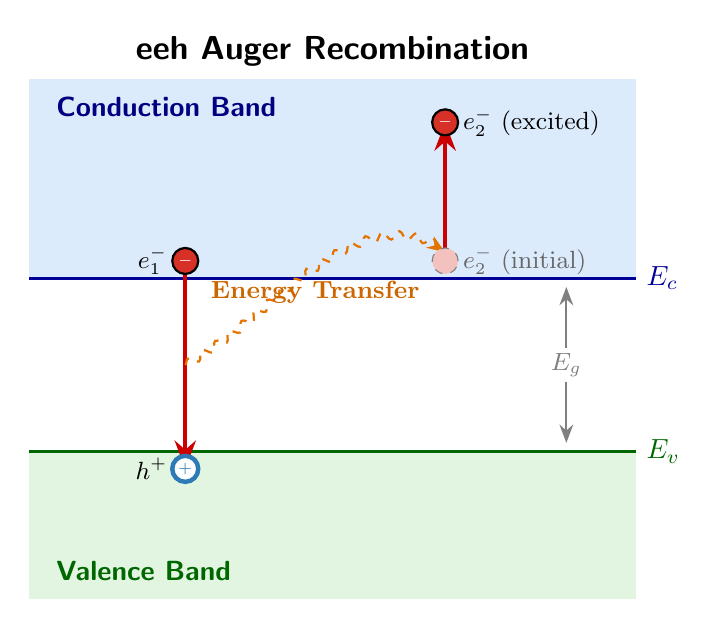
\begin{tikzpicture}[scale=1.1, >=Stealth]

    % ==========================================
    % 1. ENERGY BANDS & SHADING
    % ==========================================
    % Conduction Band (CB)
    \fill[conductionblue] (0, 2.5) rectangle (7, 4.8);
    \draw[very thick, blue!60!black] (0, 2.5) -- (7, 2.5) node[right, font=\bfseries] {$E_c$};
    \node[anchor=north west, font=\bfseries\sffamily, color=blue!50!black] at (0.2, 4.7) {Conduction Band};

    % Band Gap Label
    \draw[<->, thick, gray] (6.2, 0.6) -- (6.2, 2.4) node[midway, fill=white, inner sep=2pt, font=\small] {$E_g$};

    % Valence Band (VB)
    \fill[valencegreen] (0, -1.2) rectangle (7, 0.5);
    \draw[very thick, green!40!black] (0, 0.5) -- (7, 0.5) node[right, font=\bfseries] {$E_v$};
    \node[anchor=south west, font=\bfseries\sffamily, color=green!40!black] at (0.2, -1.1) {Valence Band};

    % ==========================================
    % 2. PARTICLES & TRANSITIONS
    % ==========================================

    % --- Process 1: e-h Recombination (Left side) ---
    % Initial Electron (e1) in CB
    \coordinate (e1_init) at (1.8, 2.7);
    % Final Hole (h1) in VB
    \coordinate (h1_init) at (1.8, 0.3);

    % Recombination transition arrow
    \draw[->, ultra thick, red!80!black] (e1_init) -- (h1_init);

    % Electron 1 marker
    \draw[fill=electronred, draw=black, thick] (e1_init) circle (0.15) node[white, font=\tiny\bfseries] {$-$};
    \node[left=3pt, font=\small] at (e1_init) {$e_1^-$};

    % Hole marker
    \draw[fill=white, draw=holeblue, ultra thick] (h1_init) circle (0.15) node[holeblue, font=\tiny\bfseries] {$+$};
    \node[left=3pt, font=\small] at (h1_init) {$h^+$};


    % --- Energy Transfer (Curved Wavy / Dashed Arrow) ---
    \draw[->, thick, dashed, orange!90!black, decorate, decoration={snake, amplitude=1.5pt, segment length=6pt}] 
        (1.8, 1.5) to[out=30, in=150] (4.8, 2.8);
    \node[above, font=\small\bfseries, color=orange!80!black] at (3.3, 2.1) {Energy Transfer};


    % --- Process 2: Secondary Electron Excitation (Right side) ---
    % Initial Electron (e2) near CB edge
    \coordinate (e2_init) at (4.8, 2.7);
    % Excited Electron (e2*) high in CB
    \coordinate (e2_final) at (4.8, 4.3);

    % Excitation transition arrow
    \draw[->, ultra thick, red!80!black] (e2_init) -- (e2_final);

    % Initial state marker (ghost/faded)
    \draw[fill=electronred!30, draw=gray, dashed] (e2_init) circle (0.15);
    \node[right=3pt, font=\small, color=gray!80!black] at (e2_init) {$e_2^-$ (initial)};

    % Final excited electron marker
    \draw[fill=electronred, draw=black, thick] (e2_final) circle (0.15) node[white, font=\tiny\bfseries] {$-$};
    \node[right=3pt, font=\small] at (e2_final) {$e_2^-$ (excited)};

    % ==========================================
    % 3. TITLE / CAPTION
    % ==========================================
    \node[anchor=north, font=\large\bfseries\sffamily] at (3.5, 5.4) {eeh Auger Recombination};

\end{tikzpicture}

}
  \end{minipage}\hfill
  \begin{minipage}{0.28\textwidth}
    \centering
    \resizebox{\textwidth}{!}{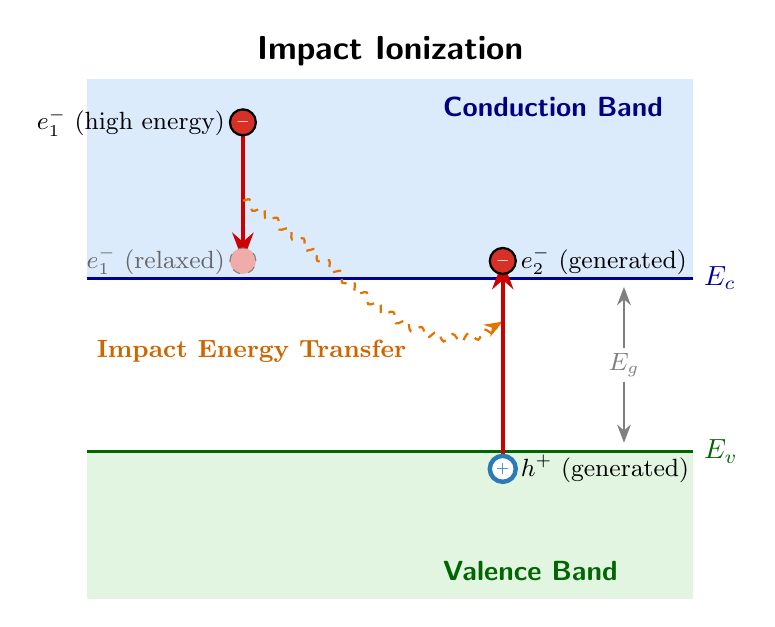
\begin{tikzpicture}[scale=1.1, >=Stealth]

    % ==========================================
    % 1. ENERGY BANDS & SHADING
    % ==========================================
    % Conduction Band (CB)
    \fill[conductionblue] (0, 2.5) rectangle (7, 4.8);
    \draw[very thick, blue!60!black] (0, 2.5) -- (7, 2.5) node[right, font=\bfseries] {$E_c$};
    \node[anchor=north west, font=\bfseries\sffamily, color=blue!50!black] at (4, 4.7) {Conduction Band};

    % Band Gap Label
    \draw[<->, thick, gray] (6.2, 0.6) -- (6.2, 2.4) node[midway, fill=white, inner sep=2pt, font=\small] {$E_g$};

    % Valence Band (VB)
    \fill[valencegreen] (0, -1.2) rectangle (7, 0.5);
    \draw[very thick, green!40!black] (0, 0.5) -- (7, 0.5) node[right, font=\bfseries] {$E_v$};
    \node[anchor=south west, font=\bfseries\sffamily, color=green!40!black] at (4, -1.1) {Valence Band};

    % ==========================================
    % 2. PARTICLES & TRANSITIONS
    % ==========================================

    % --- Process 1: High-Energy Electron Relaxation (Left side) ---
    % Initial High-Energy Electron (e1*)
    \coordinate (e1_init) at (1.8, 4.3);
    % Final Relaxed Electron (e1)
    \coordinate (e1_final) at (1.8, 2.7);

    % Relaxation transition arrow
    \draw[->, ultra thick, red!80!black] (e1_init) -- (e1_final);

    % Initial high-energy electron marker
    \draw[fill=electronred, draw=black, thick] (e1_init) circle (0.15) node[white, font=\tiny\bfseries] {$-$};
    \node[left=3pt, font=\small] at (e1_init) {$e_1^-$ (high energy)};

    % Final relaxed electron marker
    \draw[fill=electronred!40, draw=gray, dashed] (e1_final) circle (0.15);
    \node[left=3pt, font=\small, color=gray!80!black] at (e1_final) {$e_1^-$ (relaxed)};


    % --- Energy Transfer (Curved Wavy / Dashed Arrow) ---
    \draw[->, thick, dashed, orange!90!black, decorate, decoration={snake, amplitude=1.5pt, segment length=6pt}] 
        (1.8, 3.4) to[out=-30, in=-150] (4.8, 2.0);
    \node[below, font=\small\bfseries, color=orange!80!black] at (1.9, 1.9) {Impact Energy Transfer};


    % --- Process 2: Pair Generation (Right side) ---
    % Initial Valence Electron (e2) in VB
    \coordinate (e2_init) at (4.8, 0.3);
    % Final Generated Electron (e2) in CB
    \coordinate (e2_final) at (4.8, 2.7);

    % Generation transition arrow
    \draw[->, ultra thick, red!80!black] (e2_init) -- (e2_final);

    % Initial state hole creation marker (Hole left behind)
    \draw[fill=white, draw=holeblue, ultra thick] (e2_init) circle (0.15) node[holeblue, font=\tiny\bfseries] {$+$};
    \node[right=3pt, font=\small] at (e2_init) {$h^+$ (generated)};

    % Final generated electron marker in CB
    \draw[fill=electronred, draw=black, thick] (e2_final) circle (0.15) node[white, font=\tiny\bfseries] {$-$};
    \node[right=3pt, font=\small] at (e2_final) {$e_2^-$ (generated)};

    % ==========================================
    % 3. TITLE / CAPTION
    % ==========================================
    \node[anchor=north, font=\large\bfseries\sffamily] at (3.5, 5.4) {Impact Ionization};

\end{tikzpicture}

}
  \end{minipage}\hfill
  \begin{minipage}{0.30\textwidth}
    \centering
    \resizebox{\textwidth}{!}{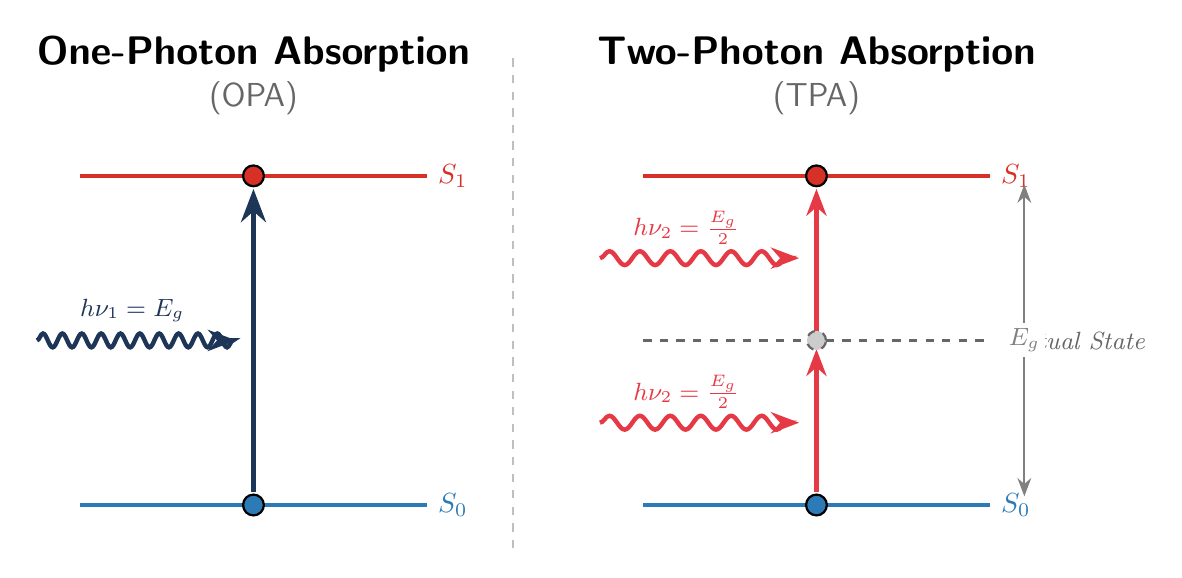
\begin{tikzpicture}[scale=1.1, >=Stealth]

    % ==========================================
    % 1. ONE-PHOTON ABSORPTION (Left Side)
    % ==========================================
    \node[font=\Large\bfseries\sffamily] at (2, 5.2) {One-Photon Absorption};
    \node[font=\large\sffamily, color=gray!80!black] at (2, 4.7) {(OPA)};

    % Energy Levels (OPA)
    \draw[ultra thick, groundstate] (0, 0) -- (4, 0) node[right, font=\bfseries] {$S_0$};
    \draw[ultra thick, excitedstate] (0, 3.8) -- (4, 3.8) node[right, font=\bfseries] {$S_1$};

    % Incoming High-Energy Photon (Blue/UV, Short Wavelength)
    \draw[->, ultra thick, photonblue, decorate, decoration={snake, amplitude=2.5pt, segment length=7pt}] 
        (-0.5, 1.9) -- (1.8, 1.9);
    \node[above, font=\small\bfseries, color=photonblue] at (0.6, 2.0) {$h\nu_1 = E_g$};

    % Vertical Transition Arrow
    \draw[->, line width=2pt, photonblue] (2, 0.15) -- (2, 3.65);

    % Electron at Ground State (Before) & Excited State (After)
    \draw[fill=groundstate, draw=black, thick] (2, 0) circle (0.12);
    \draw[fill=excitedstate, draw=black, thick] (2, 3.8) circle (0.12);


    % ==========================================
    % SEPARATOR LINE
    % ==========================================
    \draw[dashed, gray!50, thick] (5, -0.5) -- (5, 5.2);


    % ==========================================
    % 2. TWO-PHOTON ABSORPTION (Right Side)
    % ==========================================
    \node[font=\Large\bfseries\sffamily] at (8.5, 5.2) {Two-Photon Absorption};
    \node[font=\large\sffamily, color=gray!80!black] at (8.5, 4.7) {(TPA)};

    % Energy Levels (TPA)
    \draw[ultra thick, groundstate] (6.5, 0) -- (10.5, 0) node[right, font=\bfseries] {$S_0$};
    % Virtual State (Dashed Line)
    \draw[thick, dashed, gray!80!black] (6.5, 1.9) -- (10.5, 1.9) node[right, font=\small\itshape] {Virtual State};
    \draw[ultra thick, excitedstate] (6.5, 3.8) -- (10.5, 3.8) node[right, font=\bfseries] {$S_1$};

    % First Incoming Photon (Red/IR, Longer Wavelength)
    \draw[->, ultra thick, photonred, decorate, decoration={snake, amplitude=2.5pt, segment length=11pt}] 
        (6.0, 0.95) -- (8.3, 0.95);
    \node[above, font=\small\bfseries, color=photonred] at (7.0, 1.0) {$h\nu_2 = \frac{E_g}{2}$};

    % Second Incoming Photon (Red/IR)
    \draw[->, ultra thick, photonred, decorate, decoration={snake, amplitude=2.5pt, segment length=11pt}] 
        (6.0, 2.85) -- (8.3, 2.85);
    \node[above, font=\small\bfseries, color=photonred] at (7.0, 2.9) {$h\nu_2 = \frac{E_g}{2}$};

    % Vertical Transition Arrows (Two-step excitation)
    \draw[->, line width=1.5pt, photonred] (8.5, 0.15) -- (8.5, 1.8);
    \draw[->, line width=1.5pt, photonred] (8.5, 2.0) -- (8.5, 3.65);

    % Electron Positions (Ground, Virtual, Excited)
    \draw[fill=groundstate, draw=black, thick] (8.5, 0) circle (0.12);
    \draw[fill=gray!40, draw=gray!80!black, thick, dashed] (8.5, 1.9) circle (0.11);
    \draw[fill=excitedstate, draw=black, thick] (8.5, 3.8) circle (0.12);

    % Energy Gap Annotation (Right Edge)
    \draw[<->, thick, gray] (10.9, 0.1) -- (10.9, 3.7) node[midway, fill=white, inner sep=2pt, font=\small] {$E_g$};

\end{tikzpicture}
}
  \end{minipage}
\end{frame}


\begin{frame}{Carrier Two-Temperature Model}
  \begin{block}{Carrier Temperature Model}
        Carrier temperature model
    \begin{equation}
      C_{\text{c}}\pdv[]{T_{\text{c}}}{t}=-K\left(T_{\text{C}}-T_{\text{l}}\right)+\left(\alpha +\beta I +\Theta n\right)I -\pdv[]{n}{t}\left(E_{\text{g}}+3k_{\text{B}}T_{\text{c}}\right)-n\left(\pdv[]{E_{\text{g}}}{n}\pdv[]{n}{t}+\pdv[]{E_{\text{g}}}{T_{\text{c}}}\pdv[]{T_{\text{c}}}{t}\right)
     \end{equation}
  \end{block}

\end{frame}


\begin{frame}{Carrier Two-Temperature Model}
  \begin{block}{Lattice Temperature Model}
        Lattice temperature model
    \begin{equation}
      C_{\text{l}}\pdv[]{T_{\text{l}}}{t}=K\left(T_{\text{c}}-T_{\text{l}}\right)
    \end{equation}
  \end{block}

\end{frame}


\begin{frame}{Carrier Two-Temperature Model}
  \begin{block}{Drude Model}
        Drude conductivity
    \begin{equation}
      \sigma=\frac{\sigma_0}{\nu\left(T_{\text{l}}\right)}
    \end{equation}
  \end{block}

\end{frame}


\begin{frame}{Carrier Two-Temperature Model}
  \begin{figure}[!h]
    \centering
    \resizebox{0.8\textwidth}{!}{\begin{tikzpicture}
\begin{axis}[
    width=11cm,
    height=7.5cm,
    xlabel={Time $\left[\text{ps}\right]$},
    ylabel={Temperature $\left[\text{K}\right]$},
    xmin=0, xmax=10,
    ymin=200, ymax=2400,
    grid=both,
    grid style={line width=.1pt, draw=gray!20},
    major grid style={line width=.2pt, draw=gray!50},
    legend style={at={(0.55,0.77)}, anchor=north west, font=\small}
]

    % Electron Temperature (T_e)
    \addplot[line width=1.2pt, red] table[x=time_ps, y=T_e, col sep=comma] {tikz/data.csv};
    \addlegendentry{$T_e$ (Electron)}

    % Hole Temperature (T_h)
    \addplot[line width=1.2pt, orange] table[x=time_ps, y=T_h, col sep=comma] {tikz/data.csv};
    \addlegendentry{$T_h$ (Hole)}

    % Lattice Temperature (T_l)
    \addplot[line width=1.2pt, blue] table[x=time_ps, y=T_l, col sep=comma] {tikz/data.csv};
    \addlegendentry{$T_l$ (Lattice)}

\end{axis}

% Secondary Y-Axis for Carrier Density (n_e)
\begin{axis}[
    width=11cm,
    height=7.5cm,
    xmin=0, xmax=10,
    ymin=0, ymax=0.0009,
    axis y line*=right,
    axis x line=none,
    ylabel={Electron Density $\left[\cdot10^{21}\,\text{cm}^{-3}\right]$},
    ylabel style={text=teal},
    yticklabel style={text=teal, /pgf/number format/fixed, /pgf/number format/precision=4},
    legend style={at={(0.55,0.60)}, anchor=north west, font=\small}
]
    \addplot[line width=1.2pt, teal, dashed] table[x=time_ps, y= n_e, col sep=comma] {tikz/data.csv};
    \addlegendentry{$n_e$ (Carrier Density)}
\end{axis}
\end{tikzpicture}
}
  \end{figure}
\end{frame}


\section{Electrical Detection}

\begin{frame}{Electrical Detection}
  \begin{minipage}{0.48\textwidth}
    \begin{itemize}
      \item $500\,\unit{\hertz}$ modulation
      \item $1\,\unit{\kilo\hertz}$ repetition rate 
      \item Lock-in amplifier SR-830
%        \subitem \color{signalred}{Large integration time}
%        \subitem \color{signalred}{Not gated}
      \item Box car averager
%        \subitem \color{MutedSage}{Integration over many shots}
%        \subitem \color{MutedSage}{Gated}
    \end{itemize}
  \end{minipage} \hfill
  \begin{minipage}{0.48\textwidth}
    \centering
%    \includegraphics[width=\textwidth]{}
  \end{minipage}
\end{frame}


\begin{frame}{Electrical Detection}
  \centering
  \resizebox{0.8\textwidth}{!}{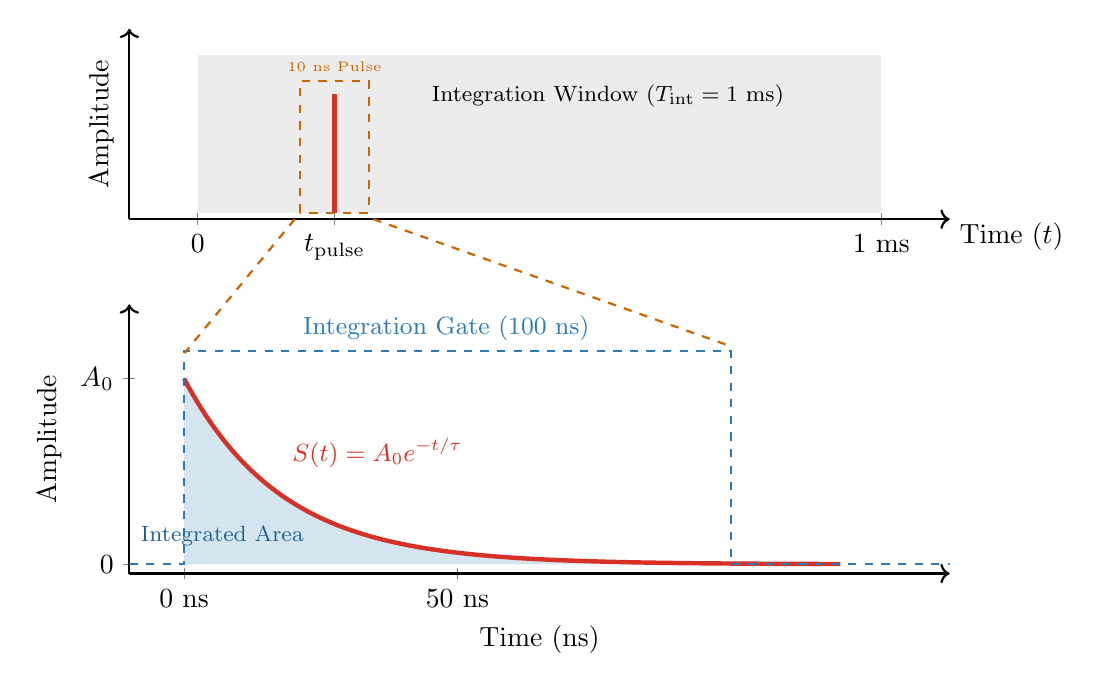
\begin{tikzpicture}
    % ==========================================
    % TOP AXIS: Macro View (1 ms Integration Window)
    % ==========================================
    \begin{axis}[
        name=macroAxis,
        width=12cm, height=4cm,
        xmin=-0.1, xmax=1.1,
        ymin=-0.05, ymax=1.4,
        axis lines=left,
        xlabel={Time ($t$)},
        ylabel={Amplitude},
        xtick={0, 0.2, 1.0},
        xticklabels={$0$, $t_{\mathrm{pulse}}$, $1\mathrm{~ms}$},
        ytick=\empty,
%        title=\textbf{Integration Window ($1\mathrm{~ms}$)},
        every axis x label/.style={at={(current axis.right of origin)},anchor=north west},
        axis line style={->, thick}
    ]
        % Integration Window background
        \fill[gray!15] (axis cs:0,0) rectangle (axis cs:1,1.2);
        \node[anchor=north] at (axis cs:0.6, 1.05) {\footnotesize Integration Window ($T_{\mathrm{int}} = 1\mathrm{~ms}$)};

        % Pulse marker
        \draw[signalred, ultra thick] (axis cs:0.2,0) -- (axis cs:0.2,0.9);
        
        % Zoom indicator circle
        \draw[dashed, orange!80!black, thick] (axis cs:0.15,0) rectangle (axis cs:0.25, 1);
            
        \node[anchor=south, orange!80!black] at (axis cs:0.2, 1) {\tiny $10\mathrm{~ns}$ Pulse};
    \end{axis}

    % ==========================================
    % BOTTOM AXIS: Micro View (50 ns Zoomed-In)
    % ==========================================
    \begin{axis}[
        name=microAxis,
        at={($(macroAxis.south west)+(0,-4.5cm)$)},
        width=12cm, height=5cm,
        xmin=-10, xmax=140,
        ymin=-0.05, ymax=1.4,
        axis lines=left,
        xlabel={Time ($\mathrm{ns}$)},
        ylabel={Amplitude},
        xtick={0, 50},
        xticklabels={$0\mathrm{~ns}$, $50\mathrm{~ns}$},
        ytick={0, 1},
        yticklabels={$0$, $A_0$},
%        title=\textbf{Zoomed View: Gated Exponential Decay ($50\mathrm{~ns}$)},
        axis line style={->, thick}
    ]
        % Filled Area under Gated Exponential Decay
        \addplot[
            domain=0:100,
            samples=100,
            fill=gateblue!20,
            draw=none
        ] {exp(-x/18)} \closedcycle;
        
        % Exponential Signal Line
        \addplot[
            domain=0:120,
            samples=150,
            signalred,
            ultra thick
        ] {exp(-x/18)};
        
        % Gate Control Signal
        \draw[gateblue, thick, dashed] (axis cs:-10, 0) -- (axis cs:0, 0) 
            -- (axis cs:0, 1.15) -- (axis cs:100, 1.15) -- (axis cs:100, 0) -- (axis cs:140, 0);

        % Annotations
        \node[gateblue, font=\small, anchor=south west] at (axis cs:20, 1.15) {Integration Gate ($100\mathrm{~ns}$)};
        \node[signalred, font=\small, anchor=west] at (axis cs:18, 0.6) {$S(t) = A_0 e^{-t/\tau}$};
        \node[font=\footnotesize, color=gateblue!80!black] at (axis cs:7, 0.15) {Integrated Area};
    \end{axis}

    % Connection Lines (Zoom effect)
    \draw[dashed, orange!80!black, thick] (2.1, 0) -- (0.7, -1.7);
    \draw[dashed, orange!80!black, thick] (3.1, 0) -- (7.6, -1.6);

\end{tikzpicture}

}
\end{frame}


\begin{frame}{Electrical Detection}
  \begin{block}{Box car}
    \begin{equation}
      A[k]=\frac{1}{N}\sum_{i=0}^{N-1}\left(Signal\left[i\right]-Background\left[i\right]\right).
    \end{equation}
  \end{block}
  \centering
  \resizebox{\textwidth}{!}{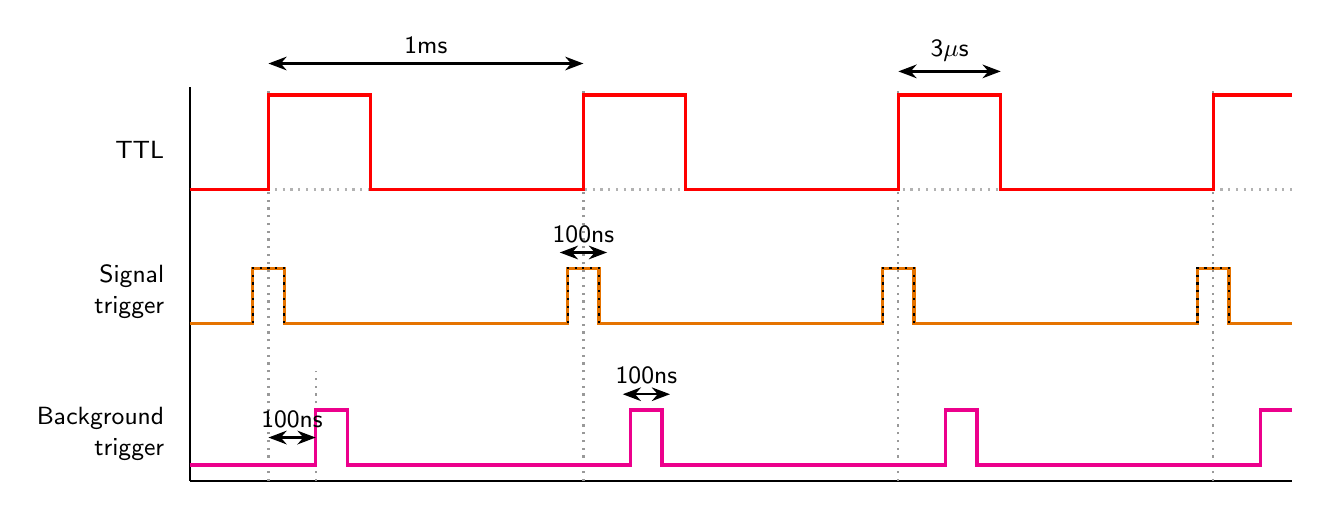
\begin{tikzpicture}[
    >=Stealth,
    font=\sffamily\small,
    axis/.style={thick},
    dottedline/.style={dotted, thick, gray!80},
    dim/.style={<->, >=Stealth, thick}
]

    % Define track vertical offsets
    \def\yTTL{3.5}
    \def\ySig{1.8}
    \def\yBg{0.0}

    % 1. Vertical Axis Baseline
    \draw[axis] (-0.5, -0.2) -- (-0.5, 4.8);

    % Horizontal Axis Baseline
    \draw[axis] (-0.5, -0.2) -- (13.5, -0.2);

    % Track Labels on the Left
    \node[left, align=right] at (-0.7, \yTTL + 0.5) {TTL};
    \node[left, align=right] at (-0.7, \ySig + 0.4) {Signal\\trigger};
    \node[left, align=right] at (-0.7, \yBg + 0.4) {Background\\trigger};

    % -------------------------------------------------------------
    % Dotted Vertical Alignment Lines & Key Coordinates
    % (Pulse positions across four repeating periods)
    % -------------------------------------------------------------
    \coordinate (t0) at (0.5, 0);
    \coordinate (t1) at (4.5, 0);
    \coordinate (t2) at (8.5, 0);
    \coordinate (t3) at (12.5, 0);

    \foreach \x in {0.5, 4.5, 8.5, 12.5} {
        \draw[dottedline] (\x, -0.2) -- (\x, 4.8);
    }

    % Additional dotted lines for background delay alignment
    \draw[dottedline] (1.1, -0.2) -- (1.1, 1.2);

    % -------------------------------------------------------------
    % 1. TTL Waveform (Red)
    % -------------------------------------------------------------
    \draw[dotted, thick, gray!60] (-0.5, \yTTL) -- (13.5, \yTTL); % Base level ref line
    \draw[red, line width=1.2pt] 
        (-0.5, \yTTL) -- (0.5, \yTTL) 
        -- (0.5, \yTTL+1.2) -- (1.8, \yTTL+1.2) -- (1.8, \yTTL) 
        -- (4.5, \yTTL) 
        -- (4.5, \yTTL+1.2) -- (5.8, \yTTL+1.2) -- (5.8, \yTTL) 
        -- (8.5, \yTTL) 
        -- (8.5, \yTTL+1.2) -- (9.8, \yTTL+1.2) -- (9.8, \yTTL) 
        -- (12.5, \yTTL) 
        -- (12.5, \yTTL+1.2) -- (13.5, \yTTL+1.2);

    % -------------------------------------------------------------
    % 2. Signal Trigger Waveform (Orange / Gold)
    % -------------------------------------------------------------
    \draw[orange!90!black, line width=1.2pt] 
        (-0.5, \ySig) -- (0.3, \ySig) 
        -- (0.3, \ySig+0.7) -- (0.7, \ySig+0.7) -- (0.7, \ySig) 
        -- (4.3, \ySig) 
        -- (4.3, \ySig+0.7) -- (4.7, \ySig+0.7) -- (4.7, \ySig) 
        -- (8.3, \ySig) 
        -- (8.3, \ySig+0.7) -- (8.7, \ySig+0.7) -- (8.7, \ySig) 
        -- (12.3, \ySig) 
        -- (12.3, \ySig+0.7) -- (12.7, \ySig+0.7) -- (12.7, \ySig) 
        -- (13.5, \ySig);

    % Dotted outline for signal pulses
    \draw[dotted, thick] (0.3, \ySig) -- (0.3, \ySig+0.7) -- (0.7, \ySig+0.7) -- (0.7, \ySig);
    \draw[dotted, thick] (4.3, \ySig) -- (4.3, \ySig+0.7) -- (4.7, \ySig+0.7) -- (4.7, \ySig);
    \draw[dotted, thick] (8.3, \ySig) -- (8.3, \ySig+0.7) -- (8.7, \ySig+0.7) -- (8.7, \ySig);
    \draw[dotted, thick] (12.3, \ySig) -- (12.3, \ySig+0.7) -- (12.7, \ySig+0.7) -- (12.7, \ySig);

    % -------------------------------------------------------------
    % 3. Background Trigger Waveform (Magenta)
    % -------------------------------------------------------------
    \draw[magenta, line width=1.2pt] 
        (-0.5, \yBg) -- (1.1, \yBg) 
        -- (1.1, \yBg+0.7) -- (1.5, \yBg+0.7) -- (1.5, \yBg) 
        -- (5.1, \yBg) 
        -- (5.1, \yBg+0.7) -- (5.5, \yBg+0.7) -- (5.5, \yBg) 
        -- (9.1, \yBg) 
        -- (9.1, \yBg+0.7) -- (9.5, \yBg+0.7) -- (9.5, \yBg) 
        -- (13.1, \yBg) 
        -- (13.1, \yBg+0.7) -- (13.5, \yBg+0.7);

    % -------------------------------------------------------------
    % Dimensions & Annotations
    % -------------------------------------------------------------

    % 1 ms Period Annotation at top
    \draw[dim] (0.5, \yTTL + 1.6) -- (4.5, \yTTL + 1.6) 
        node[midway, above] {1ms};

    % 3 us Width Annotation on TTL pulse
    \draw[dim] (8.5, \yTTL + 1.5) -- (9.8, \yTTL + 1.5) 
        node[midway, above] {3$\mu$s};

    % 100ns Pulse Width on Signal Trigger
    \draw[dim] (4.2, \ySig + 0.9) -- (4.8, \ySig + 0.9) 
        node[midway, above] {100ns};

    % 100ns Delay Annotation between TTL & Background pulse
    \draw[dim] (0.5, \yBg + 0.35) -- (1.1, \yBg + 0.35) 
        node[midway, above] {100ns};

    % 100ns Pulse Width on Background Trigger
    \draw[dim] (5.0, \yBg + 0.9) -- (5.6, \yBg + 0.9) 
        node[midway, above] {100ns};

\end{tikzpicture}

}
\end{frame}


\begin{frame}{Electrical Detection}
  \centering
  \resizebox{\textwidth}{!}{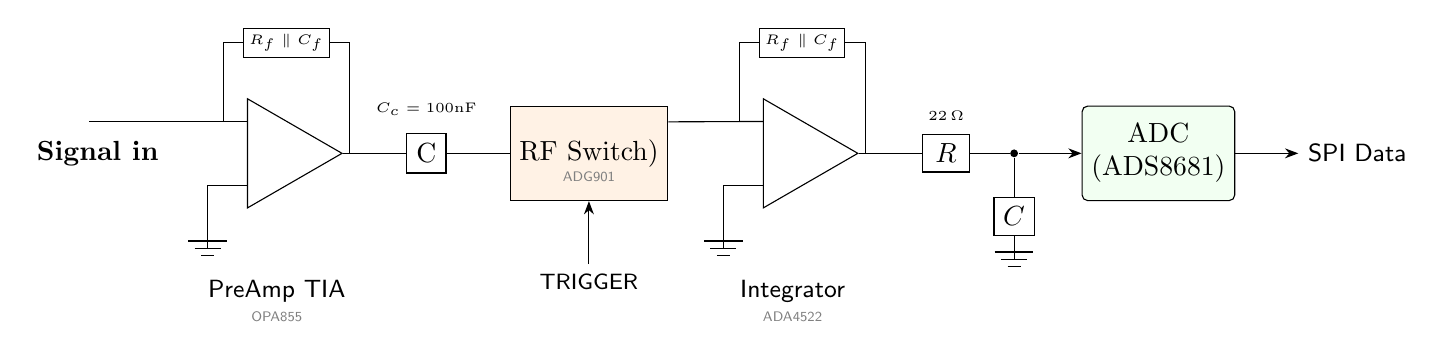
\begin{tikzpicture}[
    auto,
    node distance=1.5cm and 1.8cm,
    >=Stealth,
    circuit ee IEC, % Provides ground symbols
    % Element styles
    block/.style={draw, fill=blue!5, rectangle, minimum height=1.2cm, minimum width=1.6cm, align=center, rounded corners=2pt},
    opamp/.style={draw, fill=white, isosceles triangle, isosceles triangle apex angle=60, minimum height=1.2cm, rotate=0},
    switch/.style={draw, fill=orange!10, rectangle, minimum height=1.2cm, minimum width=1.4cm, align=center},
    label/.style={font=\sffamily\small},
    sublabel/.style={font=\sffamily\tiny\color{gray}}
]

    % 1. Signal Input
    \node (in) {\textbf{Signal in}};

    % 2. TIA Stage
    \node (tia) [right=1cm of in, opamp] {};
    \node[below=1cm of tia, label] {PreAmp TIA};
    \node[sublabel, below=1.4cm of tia] {OPA855};

    % TIA Feedback loop
    \draw (tia.left corner) + (-0.3, -0.3) -- ++(-0.3, 0.7) coordinate (tia_fb_in)
          -- ++(1.6, 0) coordinate (tia_fb_top)
          -- (tia_fb_top |- tia.apex) -- (tia.apex);
    \node[draw, fill=white, inner sep=2pt, font=\tiny] at ($(tia_fb_in)!0.5!(tia_fb_top)$) {$R_f \parallel C_f$};

    % Connections to TIA inputs
    \draw ($(tia.left corner) + (0,-0.3)$) -- ($(tia.left corner) + (-2, -0.3)$);
    \draw (tia.right corner) + (0, 0.3) -- ++(-0.5, 0.3);
    \draw (tia.right corner) + (-0.5, 0.3) -- ++(-0.5, -0.5) node[ground, rotate=-90] {};


    % 3. AC Coupling Capacitor
    \node (cap) [right=0.8cm of tia.apex, draw, fill=white, minimum width=0.5cm, minimum height=0.5cm] {C};
    \node[above=0.1cm of cap, font=\tiny] {$C_c = 100\text{nF}$};
    \draw (tia.apex) -- (cap.west);

    % 4. RF Switch (Chopper/Gate)
    \node (rfsw) [right=0.8cm of cap, switch] {RF Switch)};
    \node[sublabel, below=-0.5cm of rfsw] {ADG901};
    \draw (cap.east) -- (rfsw.west);

    % Control Trigger Input
    \node (ctrl) [below=0.8cm of rfsw, font=\sffamily\footnotesize] {TRIGGER};
    \draw[->] (ctrl) -- (rfsw.south);

    % 5. Integrator Stage
    \node (integ) [right=1.2cm of rfsw, opamp] {};
    \node[below=1cm of integ, label] {Integrator};
    \node[sublabel, below=1.4cm of integ] {ADA4522};

    % Integrator Feedback loop
    \draw (rfsw.east) + (0, 0.4) -- ($(integ.left corner) + (0, -0.3)$);
    \draw (integ.left corner) + (-0.3, -0.3) -- ++(-0.3, 0.7) coordinate (int_fb_in)
          -- ++(1.6, 0) coordinate (int_fb_top)
          -- (int_fb_top |- integ.apex) -- (integ.apex);
    \node[draw, fill=white, inner sep=2pt, font=\tiny] at ($(int_fb_in)!0.5!(int_fb_top)$) {$R_f \parallel C_f$};

   \draw (integ.right corner) + (0, 0.3) -- ++(-0.5, 0.3);
   \draw (integ.right corner) + (-0.5, 0.3) -- ++(-0.5, -0.5) node[ground, rotate=-90] {};


    % 6. RC Low Pass Filter
    \node (r_lpf) [right=0.8cm of integ.apex, draw, fill=white, minimum width=0.6cm, minimum height=0.3cm] {$R$};
    \node[above=0.05cm of r_lpf, font=\tiny] {$22\,\Omega$};
    \node (node_lpf) [right=0.5cm of r_lpf, circle, fill, inner sep=1pt] {};
    \node (c_lpf) [below=0.5cm of node_lpf, draw, fill=white, minimum width=0.4cm, minimum height=0.2cm] {$C$};
    
    \draw (integ.apex) -- (r_lpf.west);
    \draw (r_lpf.east) -- (node_lpf);
    \draw (node_lpf) -- (c_lpf.north);
    \draw (c_lpf.south) -- ++(0, -0.3) node[ground, rotate=-90] {};

    % 7. ADC Stage
    \node (adc) [right=0.8cm of node_lpf, block, fill=green!5] {ADC\\(ADS8681)};
    \draw[->] (node_lpf) -- (adc.west);

    % Signal Output Arrow
    \draw[->] (adc.east) -- ++(0.8, 0) node[right, font=\sffamily\small] {SPI Data};

\end{tikzpicture}

}
  \vspace{5mm}
  \small
  \begin{tabular}{l S[table-format=2.2] S[table-format=1.3] S[table-format=3.1]}
    \toprule
    \textbf{Component} & {\textbf{Bandwidth [GHz]}} & {\textbf{Noise [$V_{rms}/\sqrt{Hz}$]}} \\
    \midrule
    Pre-amp              & {$8$}                    & 0.342          \\
    Gated integrator     & 86.15                    & 0.281          \\
    ADC                  & 88.38                    & 0.234          \\
    \bottomrule
  \end{tabular}
\end{frame}


\begin{frame}{Electrical Detection}
  \centering
  \resizebox{\textwidth}{!}{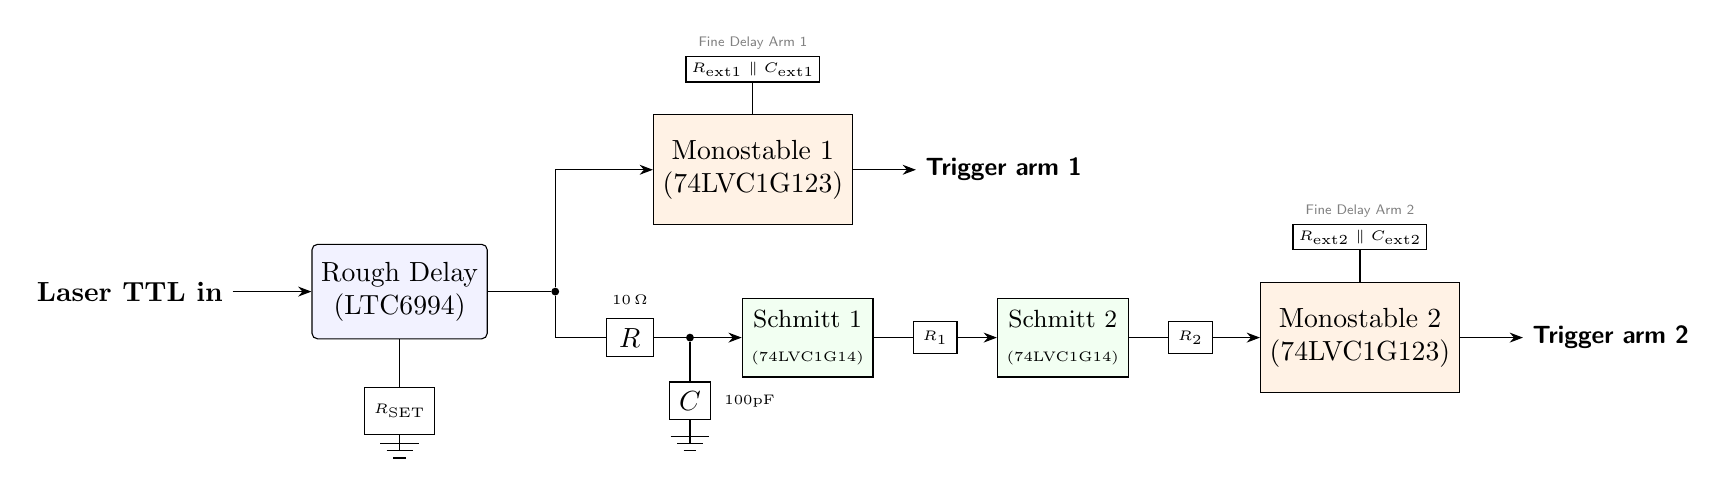
\begin{tikzpicture}[
    auto,
    node distance=1.2cm and 1.4cm,
    >=Stealth,
    circuit ee IEC,
    % Custom component styles
    block/.style={draw, fill=blue!5, rectangle, minimum height=1.2cm, minimum width=1.8cm, align=center, rounded corners=2pt},
    mono/.style={draw, fill=orange!10, rectangle, minimum height=1.4cm, minimum width=1.6cm, align=center},
    schmitt/.style={draw, fill=green!5, rectangle, minimum height=1.0cm, minimum width=1.2cm, align=center},
    label/.style={font=\sffamily\small},
    sublabel/.style={font=\sffamily\tiny\color{gray}}
]

    % 1. Input Node
    \node (in) {\textbf{Laser TTL in}};

    % 2. Rough Delay Stage (LTC6994)
    \node (rough_delay) [right=1.0cm of in, block] {Rough Delay\\(LTC6994)};
    \draw[->] (in) -- (rough_delay.west);

    % Resistor Set for LTC6994
    \node (r_set) [below=0.6cm of rough_delay, draw, fill=white, minimum width=0.4cm, minimum height=0.6cm] {\tiny $R_{\text{SET}}$};
    \draw (rough_delay.south) -- (r_set.north);
    \draw (r_set.south) -- ++(0, -0.2) node[ground, rotate=-90] {};

    % Node after Rough Delay
    \node (node_rough) [right=0.8cm of rough_delay, circle, fill, inner sep=1pt] {};
    \draw (rough_delay.east) -- (node_rough);

    % 3. First Fine Delay / Monostable (74LVC1G123 - Arm 1)
    \node (mono1) [above right=0.8cm and 1.2cm of node_rough, mono] {Monostable 1\\(74LVC1G123)};
    \node[sublabel, above=0.7cm of mono1] {Fine Delay Arm 1};

    % Passive timing network for Mono 1 (Rext1 / Cext1)
    \draw (mono1.north) -- ++(0, 0.4) coordinate (m1_tc);
    \node[draw, fill=white, inner sep=2pt, font=\tiny, above=0.0cm of m1_tc] {$R_{\text{ext1}} \parallel C_{\text{ext1}}$};

    % Connections to Mono 1
    \draw[->] (node_rough) |- (mono1.west);
    \draw[->] (mono1.east) -- ++(0.8, 0) node[right, font=\sffamily\small] {\textbf{Trigger arm 1}};

    % 4. Low-Pass Filter Stage (R_LPF3 & C_LPF3)
    \node (r_lpf) [below right=0.3cm and 0.6cm of node_rough, draw, fill=white, minimum width=0.6cm, minimum height=0.3cm] {$R$};
    \node[above=0.05cm of r_lpf, font=\tiny] {$10\,\Omega$};
    \draw (node_rough) |- (r_lpf.west);

    \node (node_lpf) [right=0.4cm of r_lpf, circle, fill, inner sep=1pt] {};
    \node (c_lpf) [below=0.5cm of node_lpf, draw, fill=white, minimum width=0.4cm, minimum height=0.2cm] {$C$};
    \node[right=0.05cm of c_lpf, font=\tiny] {100pF};

    \draw (r_lpf.east) -- (node_lpf);
    \draw (node_lpf) -- (c_lpf.north);
    \draw (c_lpf.south) -- ++(0, -0.3) node[ground, rotate=-90] {};

    % 5. Schmitt Trigger Buffers (74LVC1G14)
    \node (st1) [right=0.6cm of node_lpf, schmitt] {\small Schmitt 1\\\tiny(74LVC1G14)};
    \draw[->] (node_lpf) -- (st1.west);

    \node (r1) [right=0.5cm of st1, draw, fill=white, minimum width=0.5cm, minimum height=0.3cm] {\tiny $R_1$};
    \node (st2) [right=0.5cm of r1, schmitt] {\small Schmitt 2\\\tiny(74LVC1G14)};

    \draw (st1.east) -- (r1.west);
    \draw[->] (r1.east) -- (st2.west);

    % 6. Second Fine Delay / Monostable (74LVC1G123 - Arm 2)
    \node (r2) [right=0.5cm of st2, draw, fill=white, minimum width=0.5cm, minimum height=0.3cm] {\tiny $R_2$};
    \node (mono2) [right=0.6cm of r2, mono] {Monostable 2\\(74LVC1G123)};
    \node[sublabel, above=0.7cm of mono2] {Fine Delay Arm 2};

    % Passive timing network for Mono 2 (Rext2 / Cext2)
    \draw (mono2.north) -- ++(0, 0.4) coordinate (m2_tc);
    \node[draw, fill=white, inner sep=2pt, font=\tiny, above=0.0cm of m2_tc] {$R_{\text{ext2}} \parallel C_{\text{ext2}}$};

    \draw (st2.east) -- (r2.west);
    \draw[->] (r2.east) -- (mono2.west);

    % Final Output
    \draw[->] (mono2.east) -- ++(0.8, 0) node[right, font=\sffamily\small] {\textbf{Trigger arm 2}};

\end{tikzpicture}
}

  \small
  \begin{tabular}{l S[table-format=2.2] S[table-format=1.3] S[table-format=3.1]}
    \toprule
    \textbf{Trigger stage} & {\textbf{Imparted delay}} & {\textbf{Phase jitter [ppm/Hz]}} & {\textbf{Pulse duration}}\\
    \midrule
    Rough delay             & {$1\,\unit{\milli\second}$}                 & 0.342          & {$1\,\unit{\micro\second}$}\\
    Fine delay              & {$100\,\unit{\nano\second}$}                & 0.281          & {$1\,\unit{\micro\second}$}\\
    Trigger generation      & {$500\,\unit{\pico\second}$}                & 0.234          & {$100\,\unit{\nano\second}$}\\
    \bottomrule
  \end{tabular}
\end{frame}


\begin{frame}{Electrical Detection}

  \begin{block}{SNR formula}
    The formula for signal-to-noise ratio assuming $abc$
    \begin{equation}
      SNR = some complicated formula
    \end{equation}
  \end{block}
  
  \begin{figure}[!h]
    \centering
%    \includegraphics[width=\textwidth]{}
    \caption{}
  \end{figure}

\end{frame}


\begin{frame}{Different Photo- current/ conductivity Techniques}
  \begin{itemize}
    \item Correlation spectroscopy
    \item Vibrationally constrolled spectroscopy
    \item Near field
    \item ...?
  \end{itemize}
\end{frame}

\end{document}
